\documentclass[10pt,a4paper,onecolumn]{article}
% \usepackage[utf8]{inputenc}
\usepackage{marginnote}
\usepackage{graphicx}
\usepackage{xcolor}
\usepackage{authblk,etoolbox}
\usepackage{titlesec}
\usepackage{calc}
\usepackage{hyperref}
\usepackage{bm,array}
\hypersetup{breaklinks=true,
            bookmarks=true,
            pdfauthor=
{
      Georgios Detorakis,
  },
            pdftitle=
{
[Re] Multiple dynamical modes of thalamic relay neurons: rhythmic bursting
        and intermittent phase-locking
},
            colorlinks=true,
            citecolor=blue,
            urlcolor=blue,
            linkcolor=blue,
            pdfborder={0 0 0}}
\urlstyle{same}
\usepackage{tcolorbox}
\usepackage{ragged2e}
\usepackage{fontspec}
\usepackage{fontawesome}
\usepackage{caption}
\usepackage{listings}
\usepackage{float,lscape}
\usepackage{xcolor,colortbl}
\usepackage{amssymb,amsmath,array,amsthm}
\usepackage{marvosym}
\usepackage{array}
\usepackage[export]{adjustbox}

\newcommand{\Rm}[1]{\mathrm{#1}}

\newcolumntype{C}{>{\centering\arraybackslash}p{3.5em}}

\makeatletter
\newcommand{\thickhline}{%
    \noalign {\ifnum 0=`}\fi \hrule height 1pt
    \futurelet \reserved@a \@xhline
}
\newcolumntype{"}{@{\hskip\tabcolsep\vrule width 1pt\hskip\tabcolsep}}
\makeatother

\definecolor{Gray}{gray}{0.75}
\definecolor{LightGray}{gray}{0.95}
\lstnewenvironment{code}{\lstset{language=Haskell,basicstyle=\small\ttfamily}}{}



%\usepackage{fancyvrb}
%\VerbatimFootnotes
%\usepackage{graphicx}
%\usepackage{mdframed}
%\newmdenv[backgroundcolor=lightgray]{Shaded}


\usepackage{longtable,booktabs}

\usepackage[
  backend=biber,
%  style=alphabetic,
%  citestyle=numeric
]{biblatex}
\bibliography{detorakis-2016.bib}



% --- Macros ------------------------------------------------------------------
\renewcommand*{\bibfont}{\small \sffamily}

\definecolor{red}{HTML}{CF232B}
\newcommand{\ReScience}{Re{\bfseries \textcolor{red}{Science}}}

\newtcolorbox{rebox}
   {colback=blue!5!white, colframe=blue!40!white,
     boxrule=0.5pt, arc=2pt, fonttitle=\sffamily\scshape\bfseries,
     left=6pt, right=20pt, top=6pt, bottom=6pt}

\newtcolorbox{repobox}
   {colback=red, colframe=red!75!black,
     boxrule=0.5pt, arc=2pt, left=6pt, right=6pt, top=3pt, bottom=3pt}

% fix for pandoc 1.14     
\newcommand{\tightlist}{%
  \setlength{\itemsep}{1pt}\setlength{\parskip}{0pt}\setlength{\parsep}{0pt}}

% --- Style -------------------------------------------------------------------
\renewcommand*{\bibfont}{\small \sffamily}
\renewcommand{\captionfont}{\small\sffamily}
\renewcommand{\captionlabelfont}{\bfseries}

\makeatletter
\renewcommand\@biblabel[1]{{\bf #1.}}
\makeatother

% --- Page layout -------------------------------------------------------------
\usepackage[top=3.5cm, bottom=3cm, right=1.5cm, left=1.5cm,
            headheight=2.2cm, reversemp, includemp, marginparwidth=4.5cm]{geometry}

% --- Section/SubSection/SubSubSection ----------------------------------------
\titleformat{\section}
  {\normalfont\sffamily\Large\bfseries}
  {}{0pt}{}
\titleformat{\subsection}
  {\normalfont\sffamily\large\bfseries}
  {}{0pt}{}
\titleformat{\subsubsection}
  {\normalfont\sffamily\bfseries}
  {}{0pt}{}
\titleformat*{\paragraph}
  {\sffamily\normalsize}


% --- Header / Footer ---------------------------------------------------------
\usepackage{fancyhdr}
\pagestyle{fancy}
%\renewcommand{\headrulewidth}{0.50pt}
\renewcommand{\headrulewidth}{0pt}
\fancyhead[L]{\hspace{-1cm}\includegraphics[width=4.0cm]{rescience-logo.pdf}}
\fancyhead[C]{}
\fancyhead[R]{} 
\renewcommand{\footrulewidth}{0.25pt}

\fancyfoot[L]{\hypersetup{urlcolor=red}
              \sffamily \ReScience~$\vert$
              \href{http://rescience.github.io}{rescience.github.io}
              \hypersetup{urlcolor=blue}}
\fancyfoot[C]{\sffamily \thepage}
\fancyfoot[R]{\sffamily Sep 2015 $\vert$
                        Volume \textbf{1} $\vert$
                        Issue \textbf{1}}
\pagestyle{fancy}
\makeatletter
\let\ps@plain\ps@fancy
\fancyheadoffset[L]{4.5cm}
\fancyfootoffset[L]{4.5cm}

% --- Title / Authors ---------------------------------------------------------
% patch \maketitle so that it doesn't center
\patchcmd{\@maketitle}{center}{flushleft}{}{}
\patchcmd{\@maketitle}{center}{flushleft}{}{}
% patch \maketitle so that the font size for the title is normal
\patchcmd{\@maketitle}{\LARGE}{\LARGE\sffamily}{}{}
% patch the patch by authblk so that the author block is flush left
\def\maketitle{{%
  \renewenvironment{tabular}[2][]
    {\begin{flushleft}}
    {\end{flushleft}}
  \AB@maketitle}}
\makeatletter
\renewcommand\AB@affilsepx{ \protect\Affilfont}
%\renewcommand\AB@affilnote[1]{{\bfseries #1}\hspace{2pt}}
\renewcommand\AB@affilnote[1]{{\bfseries #1}\hspace{3pt}}
\makeatother
\renewcommand\Authfont{\sffamily\bfseries}
\renewcommand\Affilfont{\sffamily\small\mdseries}
\setlength{\affilsep}{1em}

\LetLtxMacro{\OldIncludegraphics}{\includegraphics}
\renewcommand{\includegraphics}[2][]{\OldIncludegraphics[width=12cm, #1]{#2}}


% --- Document ----------------------------------------------------------------
\title{[Re] Multiple dynamical modes of thalamic relay neurons: 
        rhythmic bursting and intermittent phase-locking}

    \usepackage{authblk}
                        \author[1]{Georgios Detorakis}
                        \affil[1]{ Department of Cognitive Sciences, UC Irvine, CA, USA}
            
\date{\vspace{-5mm}
    \sffamily \small \href{mailto:gdetorak@uci.edu}{gdetorak@uci.edu} \\
    \sffamily \small \href{mailto:gdetor@protonmail.com}{gdetor@protonmail.com}}


\setlength\LTleft{0pt}
\setlength\LTright{0pt}


\begin{document}
\maketitle

\marginpar{
  %\hrule
  \sffamily\small
  %\vspace{2mm}
  {\bfseries Editor}\\
  Name Surname\\

  {\bfseries Reviewers}\\
        Name Surname\\
        Name Surname\\
  
  {\bfseries Received}  Sep, 1, 2015\\
  {\bfseries Accepted}  Sep, 1, 2015\\
  {\bfseries Published} Sep, 1, 2015\\

  {\bfseries Licence}   \href{http://creativecommons.org/licenses/by/4.0/}{CC-BY}

  \begin{flushleft}
  {\bfseries Competing Interests:}\\
  The authors have declared that no competing interests exist.
  \end{flushleft}

  \hrule
  \vspace{3mm}

  \hypersetup{urlcolor=white}
  
    \vspace{-1mm}
  \begin{repobox}
    \bfseries\normalsize
      \href{http://github.com/rescience/rescience-submission/article}{\faGithubAlt~Article repository}
  \end{repobox}
      \vspace{-1mm}
  \begin{repobox}
    \bfseries\normalsize
      \href{http://github.com/rescience/rescience-submission/code}{\faGithubAlt~Code repository}
  \end{repobox}
        \hypersetup{urlcolor=blue}
}

\begin{rebox}
\sffamily {\bfseries A reference implementation of}
\small
\begin{flushleft}
\begin{itemize}
    \item[→] \emph{Multiple dynamical modes of thalamic relay neurons: rhythmic
        bursting and intermittent phase-locking}, Wang, X-J, Neuroscience,
        59(1), pg. 21--31, 1994.
  \end{itemize}\par
\end{flushleft}
\end{rebox}


\section{Introduction}\label{introduction}

The present paper replicates a neuron model for thalamocortical relay neurons,
proposed by X-J Wang, \cite{wang:1994}. The model is conductance-based and 
takes advantage of the interplay between a T-type calcium current and a 
non-specific cation sag current and thus, it is able to generate spindle
and delta rhythms. Another feature of this model is the presence of an
intermittent phase-locking phenomenon where action potentials of sodium take
place in a non-periodic manner, despite the fact that they are phase-locked to
the periodic input current. Finally, the model is capable of generating tonic
spike patterns. The source code for replicating Wang's model is written in
Python (Numpy, Scipy, Matplotlib, and Scikit-image).


\section{Methods}\label{methods}

In this section, a detailed description of the model is given following 
the paradigm of Nordlie et al, \cite{nordlie:2009}. To this end, a description
of the model's equations, parameters, and inputs are given in the form of
tables. 

Table~\ref{Table:1} and~\ref{Table:2} provide a description of the model and 
information about simulations duration and time steps, respectively. 
Table~\ref{Table:3} gives a glimpse of the input signals used in this work and
Table~\ref{Table:4} introduces the equations of the model. Table~\ref{Table:5}
summarizes all the parameters used in this work.

The neuron model is conductance-based, consisting of four differential
equations describing the dynamics of membrane potential and the kinetics of
a T-Type calcium current, a Sag current channel and a Potassium channel. The
rest of the currents are described by algebraic equations.
%%
\begin{table}[!htbp]
    \centering
    \begin{tabular}{ll}
        \thickhline
        \multicolumn{2}{c}{Model Summary} \\\thickhline
        \rowcolor{Gray}
        Populations  & No population -- one neuron model \\\rowcolor{LightGray}
        Topology     & -- \\ \rowcolor{Gray}
        Connectivity & -- \\ \rowcolor{LightGray}
        Neuron Model & Hodgkin-Huxley conductance-based \\\rowcolor{Gray}
        Channel Models & \\ \rowcolor{LightGray}
        Synapse Model & -- \\ \rowcolor{Gray}
        Plasticity & -- \\ \rowcolor{LightGray}
        Input & Constant current or periodic rectangular pulses \\\rowcolor{Gray}
        Measurements & Membrane potential, channels activation, phase plane \\
        \thickhline
    \end{tabular}
    \caption{{\bfseries \sffamily Summary of the model}} 
    \label{Table:1}
\end{table}
 %%  

Before proceeding to the simulations we introduce a few details regarding 
the source code and the integration method which should be accurate and fast
enough. The implementation is a Python class (Python $3.5.1$), which uses
Numpy (version $1.10.4$), Scipy (version $0.17.0$), Matplotlib
($1.5.1$) and Scikit-image (version $0.12.3$) packages. The numerical
integration is carried out using the \emph{ode} method of Scipy 
\emph{integrate} package. Three different methods were tested in this work 
(\emph{dopri5}, \emph{Adams}, \emph{BDF}, \cite{ascher:1998}). \emph{Dopri5}
is the closest numerical method to the one used by \cite{wang:1994}
(fifth-order adaptive size Runge-Kutta method). The user of the present 
implementation can choose one of the three methods at the stage of class
instantiating. For all three methods we measured spike times, membrane
potential amplitudes and the coefficient of variation using as threshold value
$0\, \Rm{mV}$. \emph{Dopri5} and \emph{Adams} methods differ in one spike 
event time whilst \emph{dopri5} and \emph{BDF} have a difference of 37 spike
events. However, all three methods (\emph{dopri5}, \emph{Adams} and \emph{BDF})
have the same $CV \simeq 2.3608$. The most striking difference is found for the
amplitude of membrane potential. Figure~\ref{Fig:1} {\bfseries \sffamily A}
shows the membrane potential (in $\Rm{mV}$) produced by \emph{dopri5} plotted 
against the membrane potential generated by \emph{Adams} method.
Figure~\ref{Fig:1} {\bfseries \sffamily B} shows the membrane potential
of a simulation using \emph{dopri5} against another using \emph{BDF}. The 
\emph{Adams} method has less differences in amplitude from \emph{dopri5} 
than \emph{BDF}. Therefore, we decided to use the \emph{Adams} method 
since it runs faster than \emph{dopri5}. 
%%
\begin{table}[!htbp]
    \centering
    \begin{tabular}{ccc}
        \thickhline
        \multicolumn{3}{c}{Simulated Time} \\ \thickhline
        Figure & Simulation Time ($\Rm{s}$) & Integration Step ($\Rm{ms}$) \\ 
        \rowcolor{LightGray}
        $1$ & $6$ & $0.05$ \\ \rowcolor{Gray}
        $2$ & $15\times \text{period}$, $5$ & $0.05$ \\ \rowcolor{LightGray}
        $3$ & $6$ & $0.05$ \\ \rowcolor{Gray} 
        $4$ & $1.5$, $1$, $1$ & $0.05$ \\ \rowcolor{LightGray} 
        $5$ & $5$ & $0.05$  \\ \rowcolor{Gray} 
        $6$ & $5$ & $0.05$  \\ \rowcolor{LightGray} 
        $7$ & $40$, $20$ & $0.05$  \\ \thickhline
    \end{tabular}
    \caption{{\bfseries \sffamily Simulated Time}}
    \label{Table:2}
\end{table}
%%  

\begin{figure}[!htbp]
    \centering
    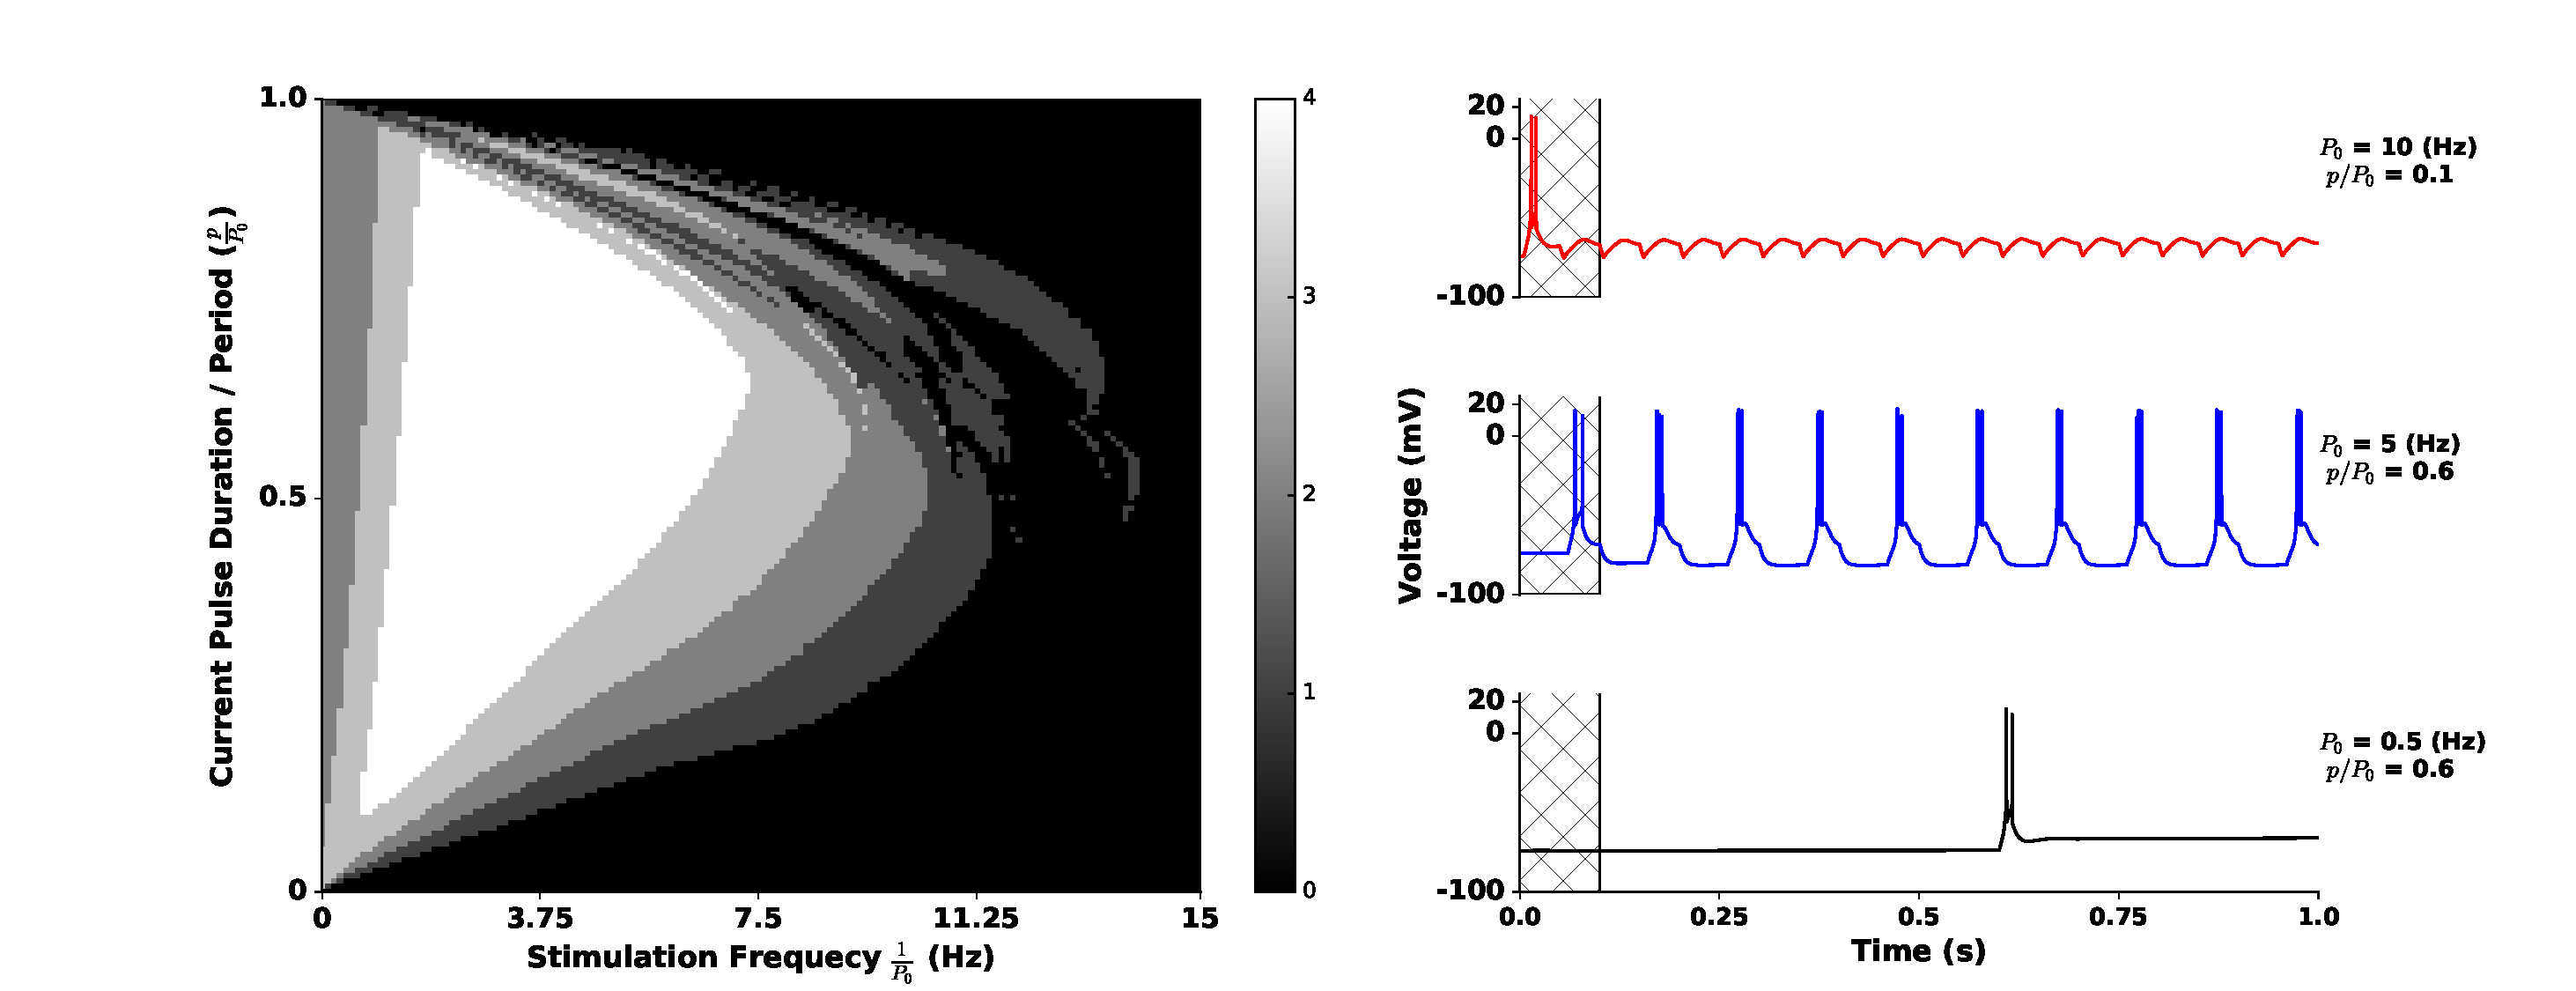
\includegraphics[width=0.9\textwidth]{figs/Figure1.pdf}
    \caption{{\bfseries \sffamily Amplitude differences} The membrane potential
    ($\Rm{mV}$) is generated using \emph{dopri5} integration method and is 
    plotted (black dots) against ({\bfseries \sffamily A}) the one generated
    by \emph{Adams} method and ({\bfseries \sffamily B}) \emph{BDF} method.
    The light shaded diagonal area indicates a $2 \, \Rm{mV}$ difference.}
    \label{Fig:1}
\end{figure}

All simulations ran on a Dell OptiPlex $7040$, equipped with a sixth
generation i$7$ processor, $8\, \Rm{GB}$ of physical memory and running Arch
Linux. The total execution time of all simulations was $526$ minutes and the
peak consumed memory was $465\, \Rm{MB}$\footnote{Python memory profiler used
    (\url{https://pypi.python.org/pypi/memory_profiler}).}\@. 
All the parameters used in this work are given in Table~\ref{Table:5}. 
%%
\begin{table}[!htbp]
    \centering
    \begin{tabular}{llcccc}
        \thickhline
        \multicolumn{6}{c}{Input} \\\thickhline
        Figure  & Type & Form & \parbox[t]{1.5cm}{Frequency
            ($\frac{1}{P_0}$, $\Rm{Hz}$)} & 
            \parbox[t]{1.5cm}{Duration ($p$, $\Rm{ms}$)} &
            \parbox[t]{1.5cm}{Amplitude ($\mu \Rm{A} / \Rm{cm}^2$)} \\
        \thickhline \rowcolor{LightGray}
        Figure~$1$ & Constant & 
            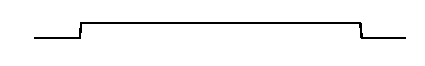
\includegraphics[width=0.1\textwidth]{figs/const.pdf} &
            -- & -- & \parbox[c]{0.3cm}{$-0.6$}
            \\\rowcolor{Gray}
        Figure~$2$ & Periodic & 
            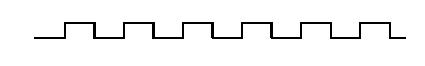
\includegraphics[width=0.1\textwidth]{figs/pulse.pdf} &
            \parbox[t]{1.1cm}{$5$, $10$} &
            \parbox[t]{1.1cm}{$10$, $40$} &
            \parbox[c]{0.3cm}{$-1.0$}
            \\\rowcolor{Gray}
        Figure~$3$ & Constant  & 
        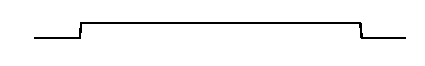
\includegraphics[width=0.1\textwidth]{figs/const.pdf} &
        -- & -- & \parbox[c]{0.3cm}{$+3.0$ \\ $3$ $0.0$ $-0.45$ $-0.455$
            $-0.47$ $-0.55$ $-0.6$ $-0.8$ $-1.3$ $-1.4$ $-2.1$} 
        \\\rowcolor{LightGray}
        Figure~$4$ & Pulse/Constant  & 
            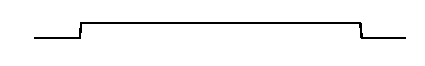
\includegraphics[width=0.1\textwidth]{figs/const.pdf} &
            -- & \parbox[c]{0.3cm}{100} & \parbox[c]{0.3cm}{$-1.25$ $0.25$ $-0.47$}
        \\\rowcolor{Gray}
        Figure~$5$ & Constant  & 
            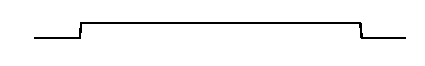
\includegraphics[width=0.1\textwidth]{figs/const.pdf} &
            -- & -- & \parbox[c]{0.3cm}{$-0.95$}
        \\\rowcolor{LightGray}
        Figure~$6$ & Constant  & 
            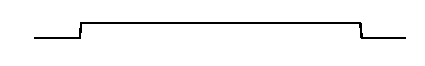
\includegraphics[width=0.1\textwidth]{figs/const.pdf} &
            -- & -- & \parbox[c]{0.3cm}{$[-2,0]$}
        \\\rowcolor{Gray}
        Figure~$7$ & Constant  & 
            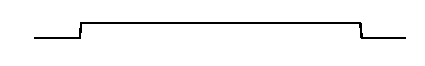
\includegraphics[width=0.1\textwidth]{figs/const.pdf} &
            -- & -- & \parbox[c]{0.3cm}{$[-2,0]$} \\
        \thickhline
    \end{tabular}
    \caption{{\bfseries \sffamily Description of the applied current
        $I_{\text{app}}$ }}
    \label{Table:3}
\end{table}
%%  

%%
\begin{table}[!htbp]
    \centering
    \begin{tabular}{p{1.5cm}ll}
        \thickhline
        \multicolumn{2}{c}{Neuron Model} \\\thickhline
        \rowcolor{Gray}
        Name  &  Thalamocortical relay neuron  \\ \rowcolor{LightGray}
        Type  &  Conductance-based neuron  \\ \rowcolor{Gray}
        Membrane Potential & $
            \begin{aligned}
                C_{\Rm{m}} \frac{dV(t)}{dt} &= -I_{\Rm{T}} - I_{\Rm{h}} - 
                I_{\Rm{Na}} - I_{\Rm{K}} - I_{\Rm{Na(P)}} - I_{\Rm{L}} +
                I_{\text{app}}
              \end{aligned}$ \\ \rowcolor{LightGray}
        T-Type Calcium Current ($I_T$) & $
            \begin{aligned}
                I_{\Rm{T}} &= g_{\Rm{T}} \cdot s^3_{\infty}(V)\cdot h \cdot
                (V-V_{\Rm{Ca}}) \\
                s_{\infty}(V) &= \frac{1}{1 + \exp(-\frac{V+65}{7.8})} \\
                \frac{dh(t)}{dt} &= \phi_h \frac{h_{\infty}(V) - h}{\tau_h(V)} \\
                h_{\infty}(V) &= \frac{1}{1 + \exp(\frac{V-\theta_h}{k_h})} \\
                \tau_h(V) &= h_{\infty}\exp(\frac{V+162.3}{17.8}) + 20
            \end{aligned} $
            \\ \rowcolor{Gray}
        Sag Current ($I_h$) & $
            \begin{aligned}
                I_h &= g_h \cdot H^2 \cdot (V-V_h) \\
                H_{\infty}(V) &= \frac{1}{1 + \exp(\frac{V+69}{7.1})} \\
                \frac{dH(t)}{dt} &= \phi_H \frac{H_{\infty}(V) - H}{\tau_H(V)} 
            \end{aligned} $
            \\ \rowcolor{LightGray} 
        Hodgkin-Huxley Currents ($I_K$) and ($I_{Na}$) & $
            \begin{aligned}
                I_{\Rm{K}} &= g_K \cdot n^4 \cdot (V - V_{\Rm{K}}) \\
                \frac{dn(t)}{dt} &= \phi_n \frac{n_{\infty}(V) - n(t)}{\tau_n(V)} \\
                n_{\infty}(\sigma_{\Rm{K}}, V) &=
                \frac{\alpha_n(\sigma_{\Rm{K}}, V)}
                {\alpha_n(\sigma_{\Rm{K}}, V) + \beta_n(\sigma_{\Rm{K}}, V)} \\
                \tau_n(\sigma_{\Rm{K}}, V) &= \frac{1}{\alpha_n(\sigma_{\Rm{K}}, V)
                + \beta_n(\sigma_{\Rm{K}}, V)} \\
                \alpha_n(\sigma_{\Rm{K}}, V) &= 
                \frac{-0.01 (V + 45.7 - \sigma_{\Rm{K}})}{\exp(-0.1(V + 45.7 - \sigma_{\Rm{K}})) - 1} \\ 
                \beta_n(\sigma_{\Rm{K}}, V) &= 0.125 \exp(-\frac{V + 55.7 -
                    \sigma_{\Rm{K}}}{80}) \\
                I_{\Rm{Na}} &= g_{\Rm{Na}} \cdot m^3_{\infty}(\sigma_{\Rm{Na}}, V)
                \cdot (0.85 - n) \cdot (V - V_{\Rm{Na}}) \\
                m_{\infty}(V) &= \frac{\alpha_m(\sigma_{\Rm{Na}}, V)}
                {\alpha_m(\sigma_{\Rm{Na}}, V) + \beta_m(\sigma_{\Rm{Na}}, V)} \\
                \alpha_m(\sigma_{\Rm{Na}}, V) &= -0.1 \frac{V + 29.7 -
                    \sigma_{\Rm{Na}}}
                    {\exp(-0.1(V + 54.7 - \sigma{\Rm{Na}})) - 1} \\
                    \beta_m(\sigma_{\Rm{Na}}, V) &=
                    4\exp(-\frac{V+54.7-\sigma_{\Rm{Na}}}{18})
            \end{aligned} $ \\ \rowcolor{Gray} 
        Persistent Sodium Currents ($I_{Na(P)}$) & $
                \begin{aligned}
                    I_{\Rm{Na(P)}} &= g_{\Rm{Na(P)}} \cdot
                    m^3_{\infty}(\sigma_{\Rm{Na(P)}},
                    V) \cdot (V - V_{\Rm{Na}}) \\
                \end{aligned} $
            \\ \rowcolor{LightGray}
        Leak Current ($I_L$) &  $
            \begin{aligned}
                I_L &= g_L \cdot (V - V_L) \\
            \end{aligned} $ \\ \thickhline
    \end{tabular}
    \caption{{\bfseries \sffamily Description of the neuron model}} 
    \label{Table:4}
\end{table}
%%

%%
\begin{table}[!htbp]
    \centering
    %\begin{tabular}{cccccccc}
    \begin{tabular}{CCCCCCCC}
        \thickhline
        \multicolumn{8}{c}{Model Parameters} \\\thickhline
        Figure & \begin{tabular}[x]{@{}c@{}} $V_0$ \\ $(\Rm{mV})$ \end{tabular}
            & \begin{tabular}[x]{@{}c@{}} $g_T$ \\ $(\Rm{mS/cm^2})$ \end{tabular}
            & \begin{tabular}[x]{@{}c@{}} $\theta_h$ \\ $(\Rm{mV})$ \end{tabular}& 
            \begin{tabular}[x]{@{}c@{}} $k_h$ \\ $(\Rm{mV^{-1}})$ \end{tabular}&
            \begin{tabular}[x]{@{}c@{}} $\sigma_{Na}$ \\ $(\Rm{mV})$ \end{tabular}&
            \begin{tabular}[x]{@{}c@{}} $g_L$ \\ $(\Rm{mS/cm^2})$ \end{tabular}&
            \begin{tabular}[x]{@{}c@{}} $V_L$ \\ $(\Rm{mV})$ \end{tabular}\\\rowcolor{LightGray}
        \thickhline
        $1$ & $-74$ & $1$ & $-79$ & $5$ & $6$ & $0.12$ & $-70$ \\\rowcolor{Gray}
        $2$ & $-74$ & $0.3$ & $-81$ & $6.25$ & $3$ & $0.1$ & $-72$ \\\rowcolor{LightGray}
        $3$ & $-74$ & $1$ & $-79$ & $5$ & $6$ & $0.12$ & $-70$ \\\rowcolor{Gray}
        $4$ & $-72$/$-64$ & $1.0$ & $-79$ & $5$ & $6$ & $0.12$ & $-70$ \\\rowcolor{LightGray}
        $5$ & $-74$ & $1.0$ & $-75$ & $5$ & $6$ & $0.08$ & $-70$ \\\rowcolor{Gray}
        $6$ & $-74$ & $1$/$0.7$ & $-79$ & $5$ & $6$ & $0.12$/$0.04$ & $-70$ \\\rowcolor{LightGray}
        $7$ & $-72$ & $0.3$/$0.25$ & $-81$ & $6.25$ & $3$ & $0.1$ & $-72$ \\
        \thickhline
        \multicolumn{8}{l}{Common Parameters} \\\rowcolor{LightGray}
        \thickhline
        \multicolumn{8}{p{36.5em}}{
        $C_m = 1\, \Rm{\mu F/cm^2}$, $\phi_h = 2$,
        $V_{\Rm{Ca}} = 120\, \Rm{mV}$, $\phi_H = 1$, $g_h = 0.04\,
        \Rm{mS/cm^2}$, $V_h = -40\, \Rm{mV}$,         
        $g_{\Rm{K}} = 30\, \Rm{mS/cm^2}$,
        $V_{\Rm{K}} = -80\, \Rm{mV}$, $g_{\Rm{Na}} = 42\,\Rm{mS/cm^2}$, 
        $V_{\Rm{Na}} = 55\, \Rm{mV}$, $\phi_{n} = \frac{200}{7}$,}\\\rowcolor{LightGray}
        \multicolumn{8}{p{36.5em}}{
        $\sigma_{\Rm{K}} = 10\, \Rm{mV}$, $V_{\Rm{Na(P)}} = 55\, \Rm{mV}$,
        $\sigma_{\Rm{Na(P)}} = -5\, \Rm{mV}$, $g_{\Rm{Na(P)}} = 9 \,
        \Rm{mS/cm^2}$}
        \\\thickhline
    \end{tabular}
    \caption{\bfseries \sffamily Simulation Parameters}
    \label{Table:5}
\end{table}
%%

\section{Results}\label{results}

We simulated the model described in Table~\ref{Table:4} using parameters
given in Table~\ref{Table:5} and the corresponding inputs (see 
Table~\ref{Table:3}). First, we examined the response of the present 
implementation to rhythmic hyperpolarization. In \cite{wang:1994} this is 
illustrated in Wang's Fig~$1$. Thus, we applied a periodic current pulse of
$-1\,\Rm{\mu A/cm^2}$ amplitude at several different frequencies
($\frac{1}{P_0}$ is the frequency in $\Rm{Hz}$ and $P_0$ is the corresponding
period in $\Rm{ms}$) ranging from $0.1\,\Rm{Hz}$ to $15\,\Rm{Hz}$ with a 
resolution (discretization) of $100$ samples. The same number of samples used 
for discretizing the duration (ON/OFF) of the pulse for each frequency. The ON
duration of a pulse is defined by the value of $p$ and the OFF duration as
$P_0 - p$. 

The results are depicted in Figure~\ref{Fig:2}. Upper panel shows two different
simulations of the present implementation at specific frequencies 
($5,\, 0.5\, \Rm{Hz}$) and ratios $p/P_0$ ($0.6, 0.6$), respectively (following
the upper panels of Fig~$1$ in \cite{wang:1994}). The results in
Figure~\ref{Fig:2} are comparable to the ones presented in \cite{wang:1994}
and the timescales are exactly the same ($400\, \Rm{ms}$ for the left sub-panel
and $4\, \Rm{s}$ for the second one). However, numbers regarding pulse ON 
duration ($p$) in Wang's Fig~$1$ are possibly an error. As an example, assume
that the frequency is $\frac{1}{P_0} = 5\, \Rm{Hz}$ and $\frac{p}{P_0} = 0.6$
then the pulse ON duration must be $p = 120\, \Rm{ms}$ and not $160\, \Rm{ms}$ 
(that is reported in \cite{wang:1994}). Bottom panel illustrates the total 
results of $100 \times 100$ simulations. In order to create this figure, we
counted the number of spikes, both supra- and sub-threshold ones, generated per
pulse and then we computed the mean (this procedure is not described 
in full detail in \cite{wang:1994}, however more details can be found in
\cite{mccormick:1990}). Figure~\ref{Fig:2} differs from the one in 
\cite{wang:1994}, to the point that the shaded area that contains an average
number of spikes below $1.0$ (but not 
zero) is larger than in \cite{wang:1994}. Unfortunately, there are not enough
details regarding Fig~$1$ in \cite{wang:1994} to make a faithful reproduction
of that figure. 

%%
\begin{figure}[!htbp]
    \centering
    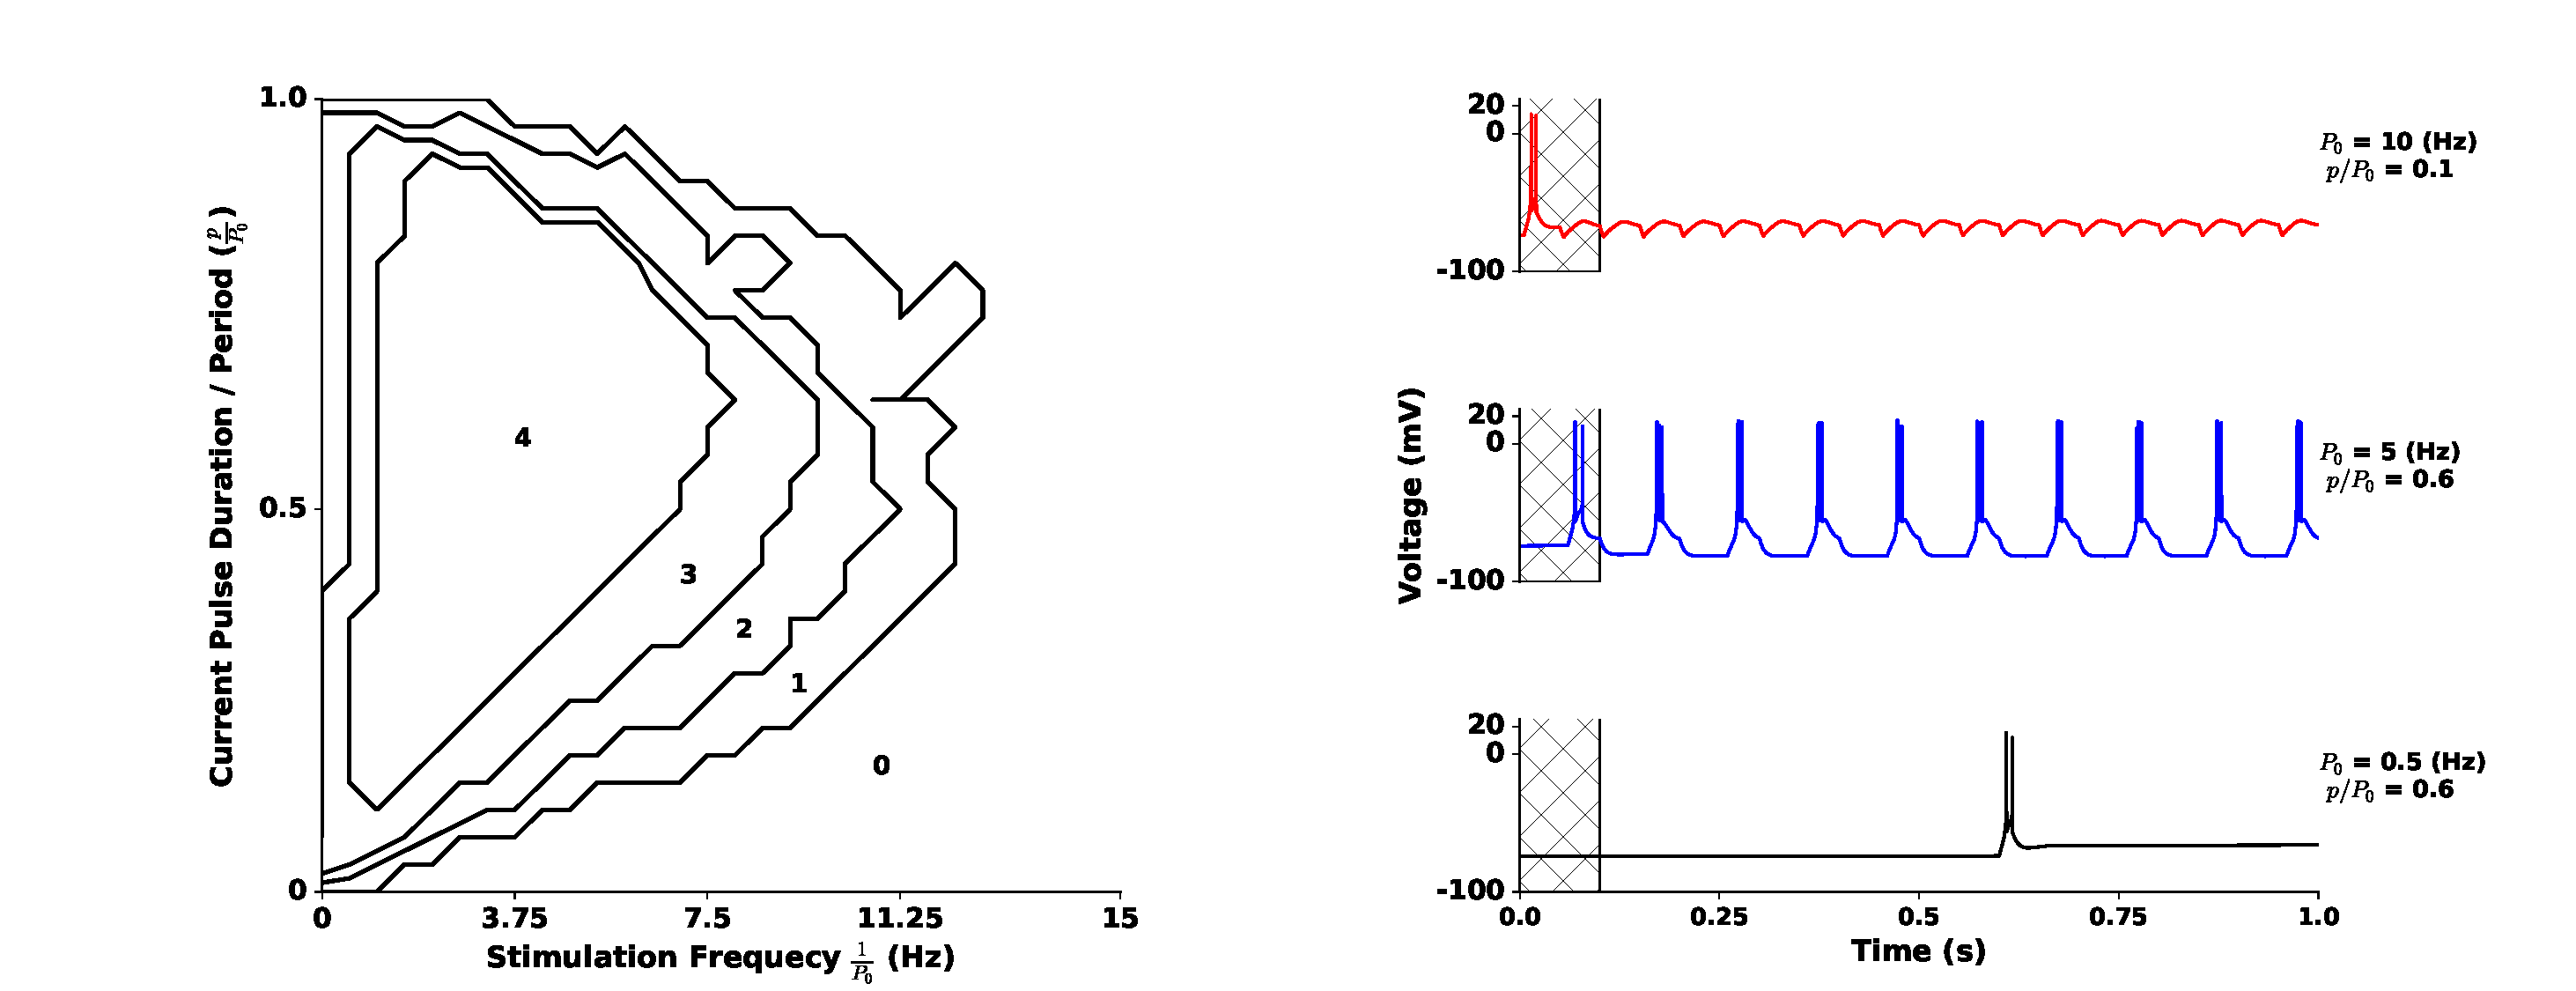
\includegraphics[width=0.6\textwidth]{figs/Figure2.pdf}
    \caption{{\bfseries \sffamily Responses to rhythmic hyperpolarizations.}
    We stimulate the model given in Table~\ref{Table:4} using a periodic pulse
    with frequency ($\frac{1}{P_0}$) varying from $0.1$ to $15\, \Rm{Hz}$.
    {\bfseries \sffamily Upper panels} show the results of two simulations out
    of $100 \times 100$. The blue curve indicates bursts of four spikes
    ($\frac{1}{P_0} = 5\, \Rm{Hz}$ and $\frac{p}{P_0} = 0.6$). Black curve
    depicts a case of two spikes bursts ($\frac{1}{P_0} = 0.5\, \Rm{Hz}$ and
    $\frac{p}{P_0} = 0.6$).
    {\bfseries \sffamily Bottom panel} shows the average number of spikes (sub-
    or supra-threshold) measured per pulse. Frequency varies in the interval 
    $[0.1, 15]\, \Rm{Hz}$ and the ratio $\frac{p}{P_0}$ is in interval $[0, 1]$.
    Numbers signify the average number of spikes per pulse.}
    \label{Fig:2}
\end{figure}
%%

The next simulation investigated the transition from subthreshold to bursting
oscillations via chaos. This is illustrated in Fig~$3$ in \cite{wang:1994}. In
this case a steady current is applied to the model described in
Table~\ref{Table:4}. In \cite{wang:1994} Wang used eleven different
amplitudes for the constant current in order to explore the model's behavior
repertoire. Hence, 
$$I_{\text{app}} = 
3.0, 0.0, -0.45, -0.455, -0.47, -0.55, -0.6, -0.8, -1.3, -1.4, -2.0\, 
\Rm{\mu A /cm^2}.$$
The results for these simulations are depicted in Figure~\ref{Fig:3}. In this
case, there was no difference between the present implementation and the
original one.
%%
\begin{figure}[!htbp]
    \centering
    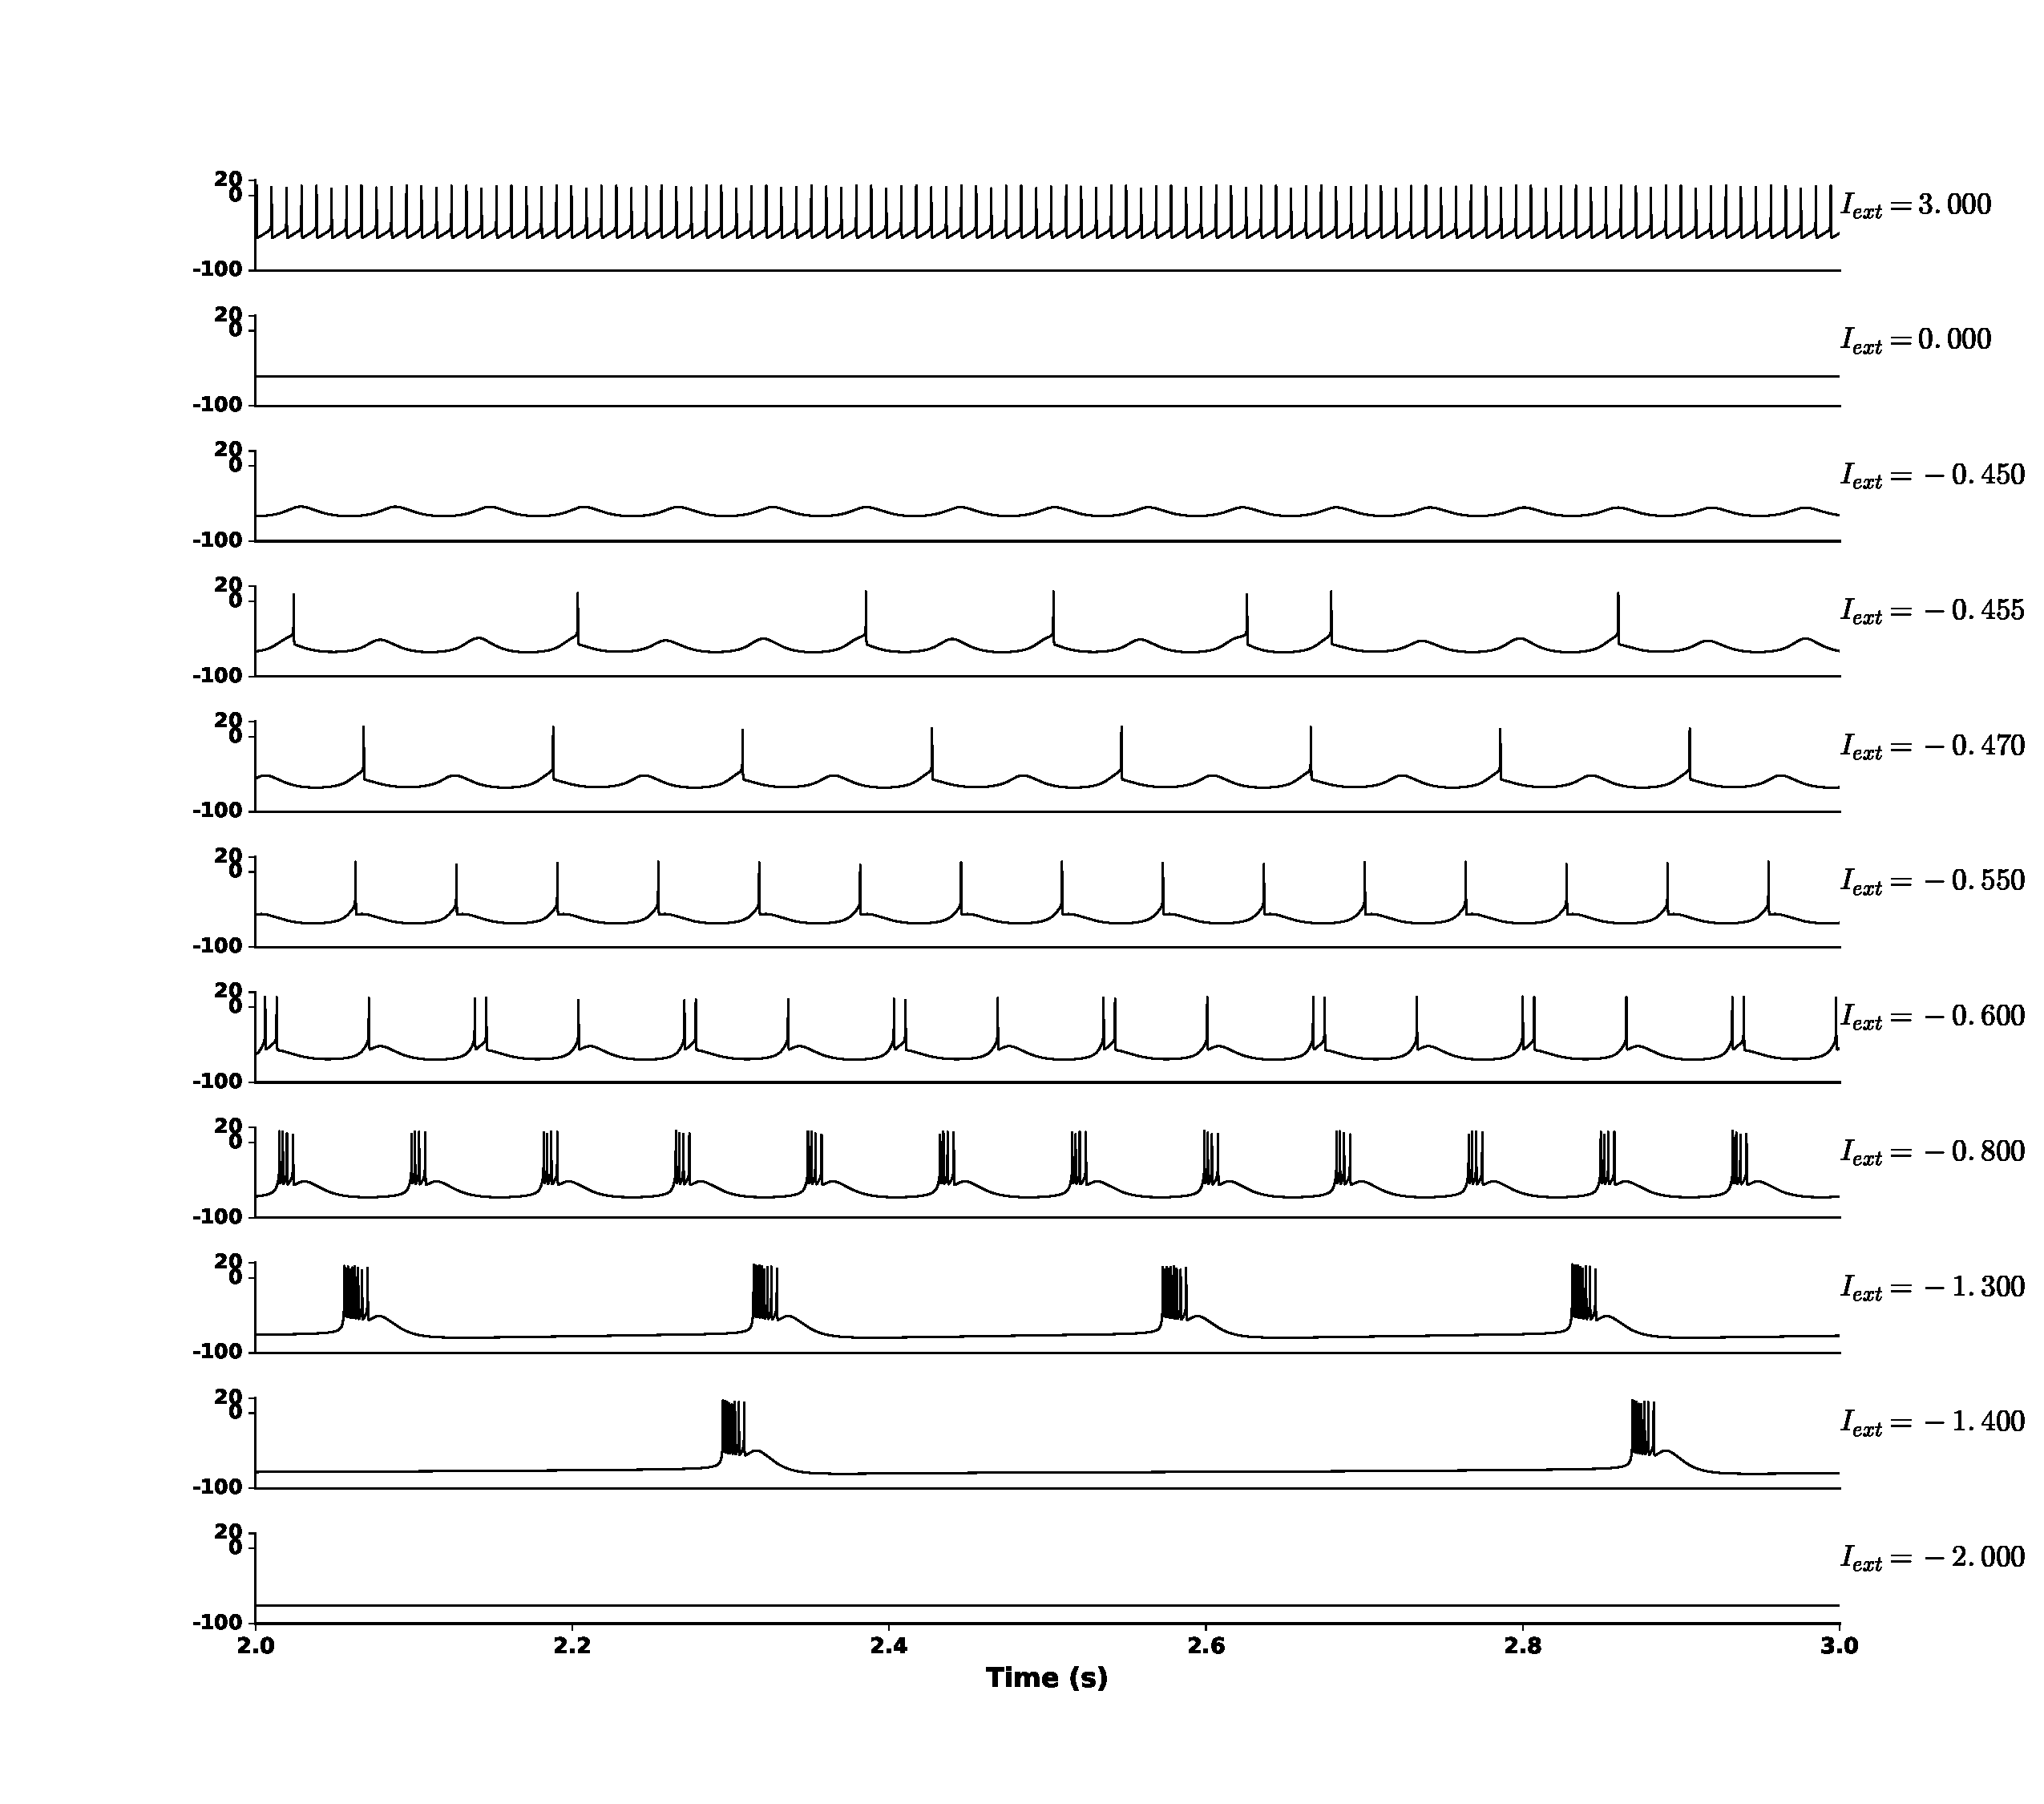
\includegraphics[width=1.\textwidth]{figs/Figure3.pdf}
    \caption{{\bfseries \sffamily Dynamic behavior of neuron.} 
    Eleven different external constant currents $I_{\text{app}} = 
    3.0, 0.0, -0.45, -0.455, -0.47, -0.55, -0.6, -0.8, -1.3, -1.4, -2.0\, 
    \Rm{\mu A /cm^2}$ have been applied as inputs to the model described by
    equations given in Table~\ref{Table:4}. The behavior of the model spans
    from tonic spiking to spikes bursts, subthreshold activity and no activity 
    at all.}
    \label{Fig:3}
\end{figure}
%%

\cite{wang:1994} has showed that the current model expresses a hysteresis
(see Wang's Fig~$4$). In order to reproduce that case we simulated
the model using a constant external current $I_{app}$. The simulation starts
by applying a current with an amplitude of $-0.433\, \Rm{\mu A / cm^2}$ and 
continues by increasing the amplitude up to $-0.55 \mu A /cm^2$. At every 
iteration, sub- and/or supra-threshold activity of the membrane potential is 
detected. The results are given in Figure~\ref{Fig:4} {\bfseries \sffamily A}. 
%%
\begin{figure}[!htbp]
    \centering
    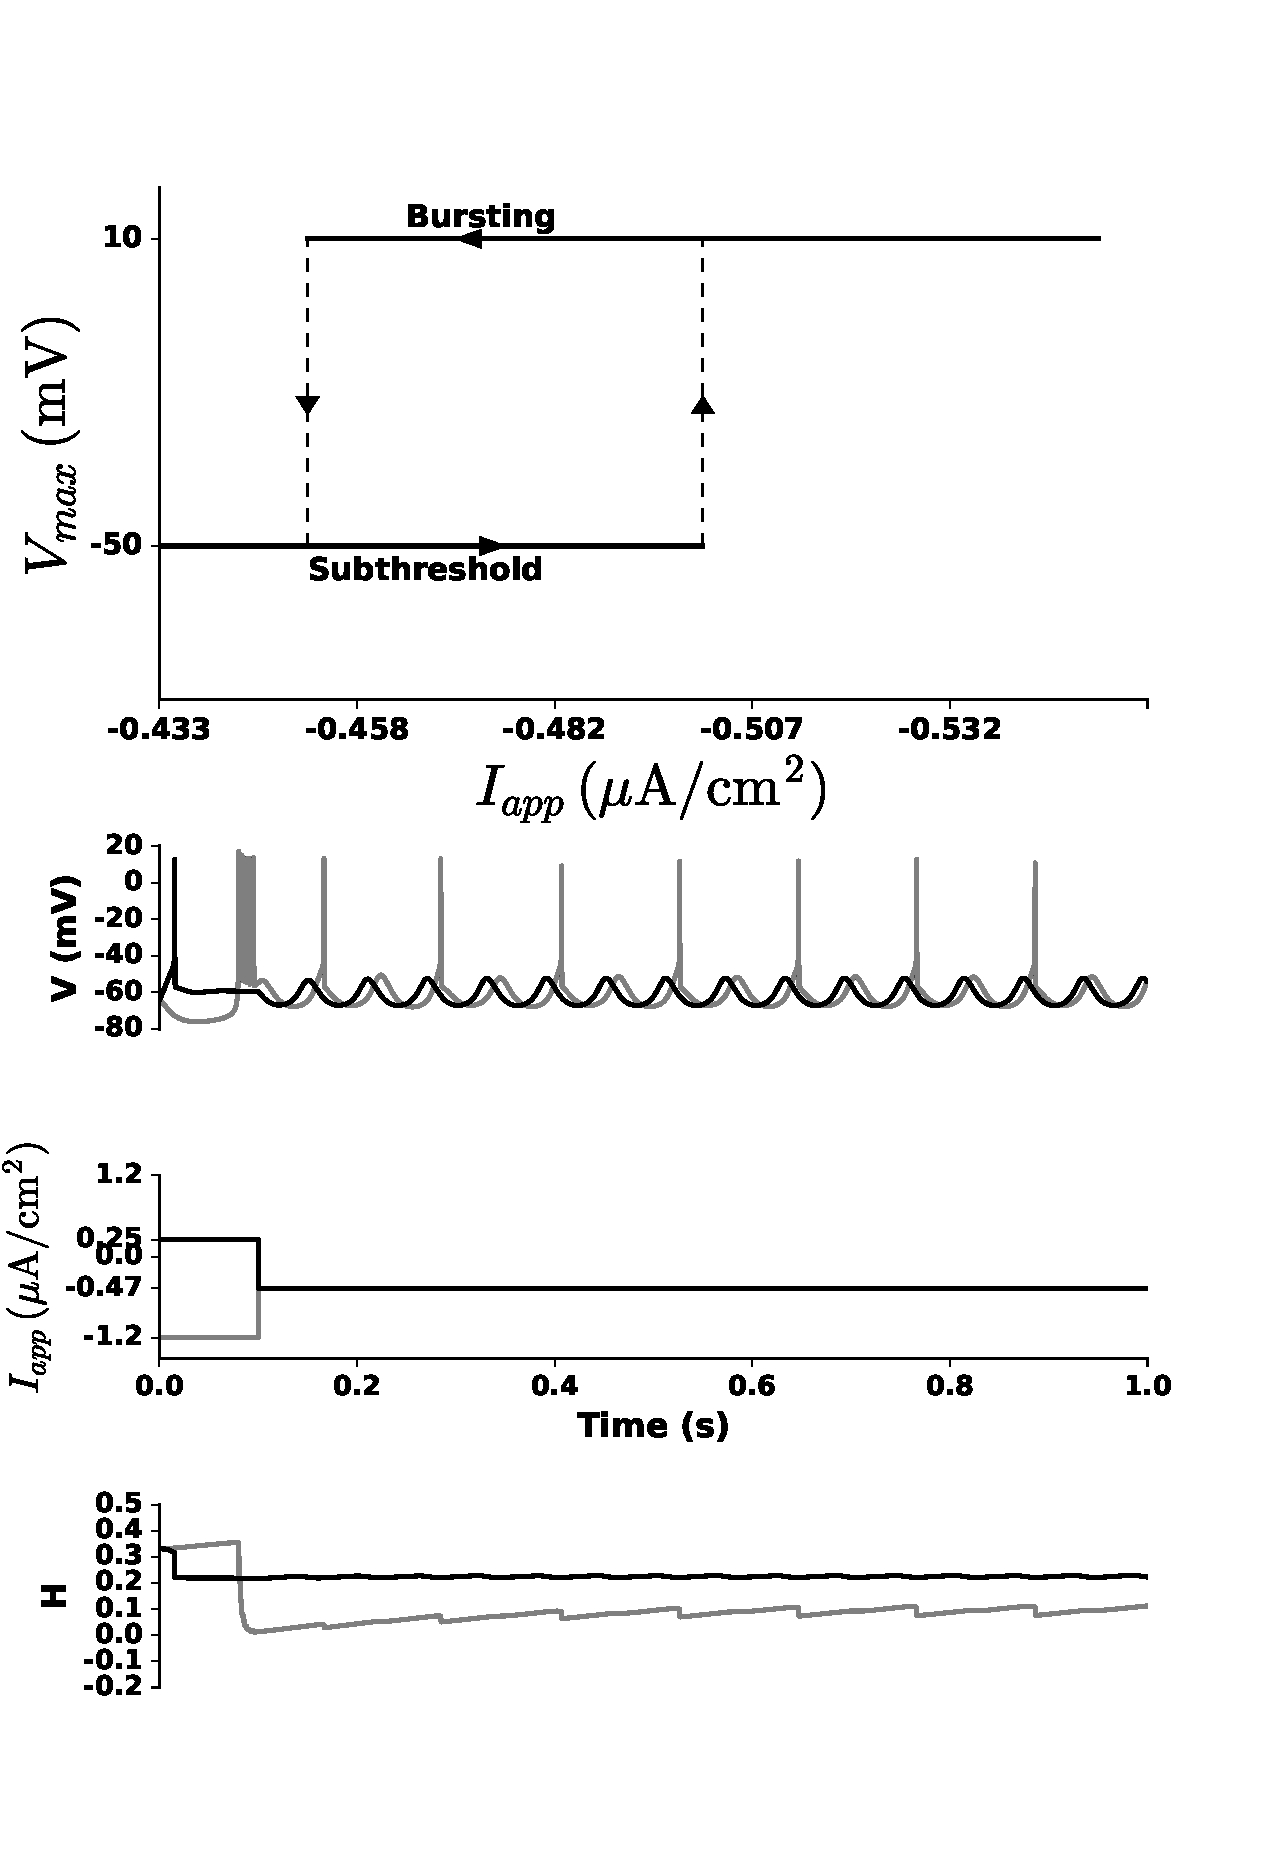
\includegraphics[width=0.6\textwidth]{figs/Figure4.pdf}
    \caption{{\bfseries \sffamily Hysteresis near the transition from the
    subthreshold to bursting oscillation.} ({\bfseries \sffamily A})
    Hysteresis diagram indicates a coexistence of bursting and subthreshold 
    activity. ({\bfseries \sffamily B}) Bistability example
    shows how the same system can produce either subthreshold activity (black
    curve) or burst activity (gray curve). ({\bfseries \sffamily C}) shows the
    activation of $H$ for the same simulation as in the 
    panel above. ({\bfseries  \sffamily D}) A brief current pulse at
    $0.25\, \Rm{\mu A /cm^2}$ (black curve) or $-1.2\, \Rm{\mu A/cm^2}$ (gray
    curve) followed by a steady current at $-0.47\, \Rm{\mu A/cm^2}$ is used 
    as external input to the model. }
    \label{Fig:4}
\end{figure}
%%
In addition, the model expresses a bistability. This was tested by applying the
same protocol as in \cite{wang:1994}. Thus first a brief pulse 
(for $100\, \Rm{ms}$) of $0.25\, \Rm{\mu A /cm^2}$ (black line in
Figure~\ref{Fig:4} {\bfseries \sffamily C}) or $-1.2\, \Rm{\mu A/cm^2}$ (gray
line in Figure~\ref{Fig:4} {\bfseries \sffamily C}) is applied to the model
followed by a steady current at $-0.47\, \Rm{\mu A /cm^2}$. Such a protocol
causes the state of the model to switch from purely sub-threshold to mixed
sub- and suprathreshold. These results are illustrated in
Figure~\ref{Fig:4} {\bfseries \sffamily B}. In
the same figure panels {\bfseries \sffamily C} and {\bfseries \sffamily D}
depict the input to the model and the $H$ of the Sag channel, respectively. 

Another interesting behavior of the model is the development of ``spiral''
chaos (see Fig~$6$ in \cite{wang:1994}). In this case the external input 
is constant and its amplitude is set to $-0.95\, \Rm{\mu A / cm^2}$. The
results for this case are shown in Figure~\ref{Fig:5}, and the current model
is capable of generating ``spiral'' chaos as in \cite{wang:1994}. 
%%
\begin{figure}[!htbp]
    \centering
    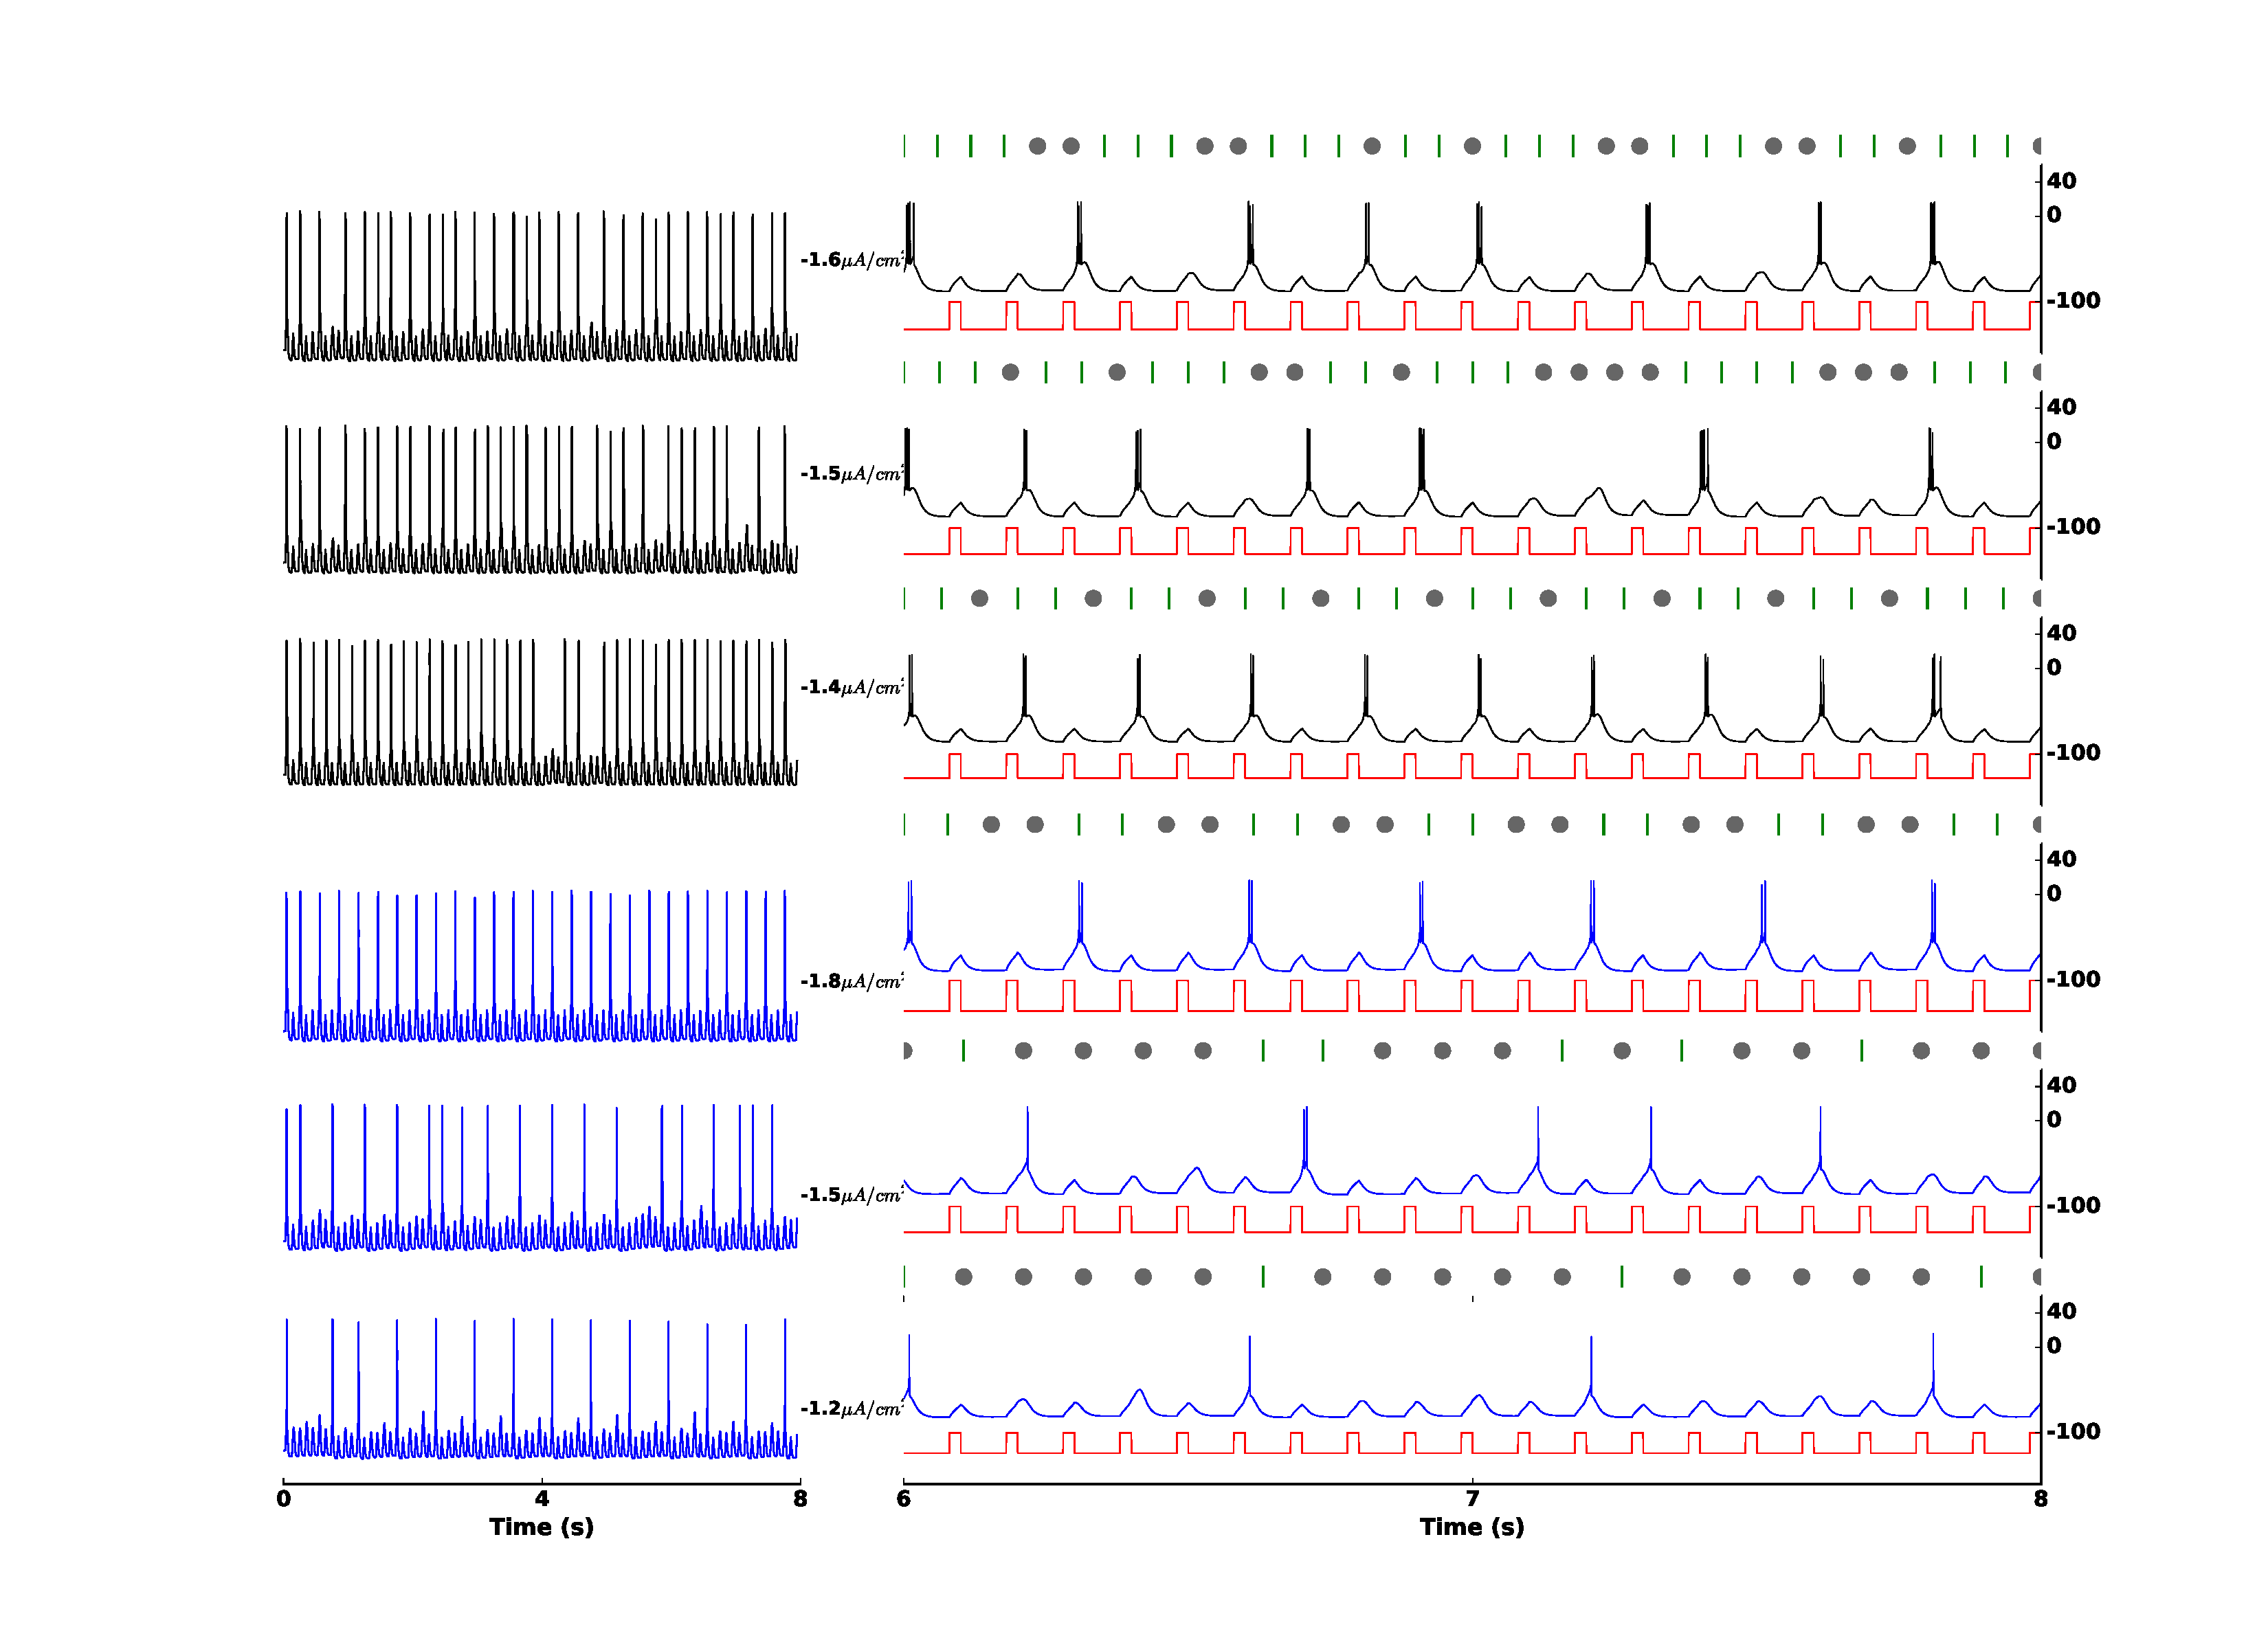
\includegraphics[width=.6\textwidth]{figs/Figure5.pdf}
    \caption{{\bfseries \sffamily ``Spiral Chaos''.} It is generated when a
    constant current with amplitude $-0.95\Rm{\mu A/cm^2}$ is injected to the 
    model described in Table~\ref{Table:4} and using the parameters from
    Table~\ref{Table:5}. {\bfseries \sffamily Top panel} shows the phase
    portrait of the membrane potential and the Sag current ($V$ vs $h$).
    {\bfseries \sffamily Middle panel} illustrates the membrane potential ($V$)
    and, the {\bfseries \sffamily bottom panel} shows the $h$ current over time.}
    \label{Fig:5}
\end{figure}
%%

The bursting frequency of the model can be affected by the injected external
current (see Fig~$7$ in \cite{wang:1994}, two bursting modes). To verify that
the present implementation is capable of producing similar results we 
captured data\footnote{Data are available in the accompanying github repository
of the present article.} values for the external current from Fig~$7$ of the 
original article (dots in Fig $7$, pg. $27$ in \cite{wang:1994}) using a 
software called PlotDigitizer\footnote{\url{(http://plotdigitizer.sourceforge.net/})}.
So for every data point (external current amplitude), we ran a simulation and
the bursting frequency of the membrane potential was measured. The results are
illustrated in Figure~\ref{Fig:6}. The black curve shows the frequency in 
$\Rm{Hz}$ and the blue curve shows the period in $\Rm{sec}$. Black dots indicate
the frequency and open circles the corresponding period (present implementation),
respectively. Cyan crosses show the original data taken from \cite{wang:1994} 
and magenta pentagons the corresponding period. It is apparent that the
present implementation is able to reproduce Wang's Fig~$7$, despite the fact
that some of the original points do not match the exactly the ones computed
using the reference implementation code. Furthermore, it is worth mentioning 
that for properly replicate Figure~\ref{Fig:6} we had to run quite long
simulations (see Table~\ref{Table:2}). If the signal is too short the results 
can be quite different from the ones given in \cite{wang:1994}.
%%
\begin{figure}[!htbp]
    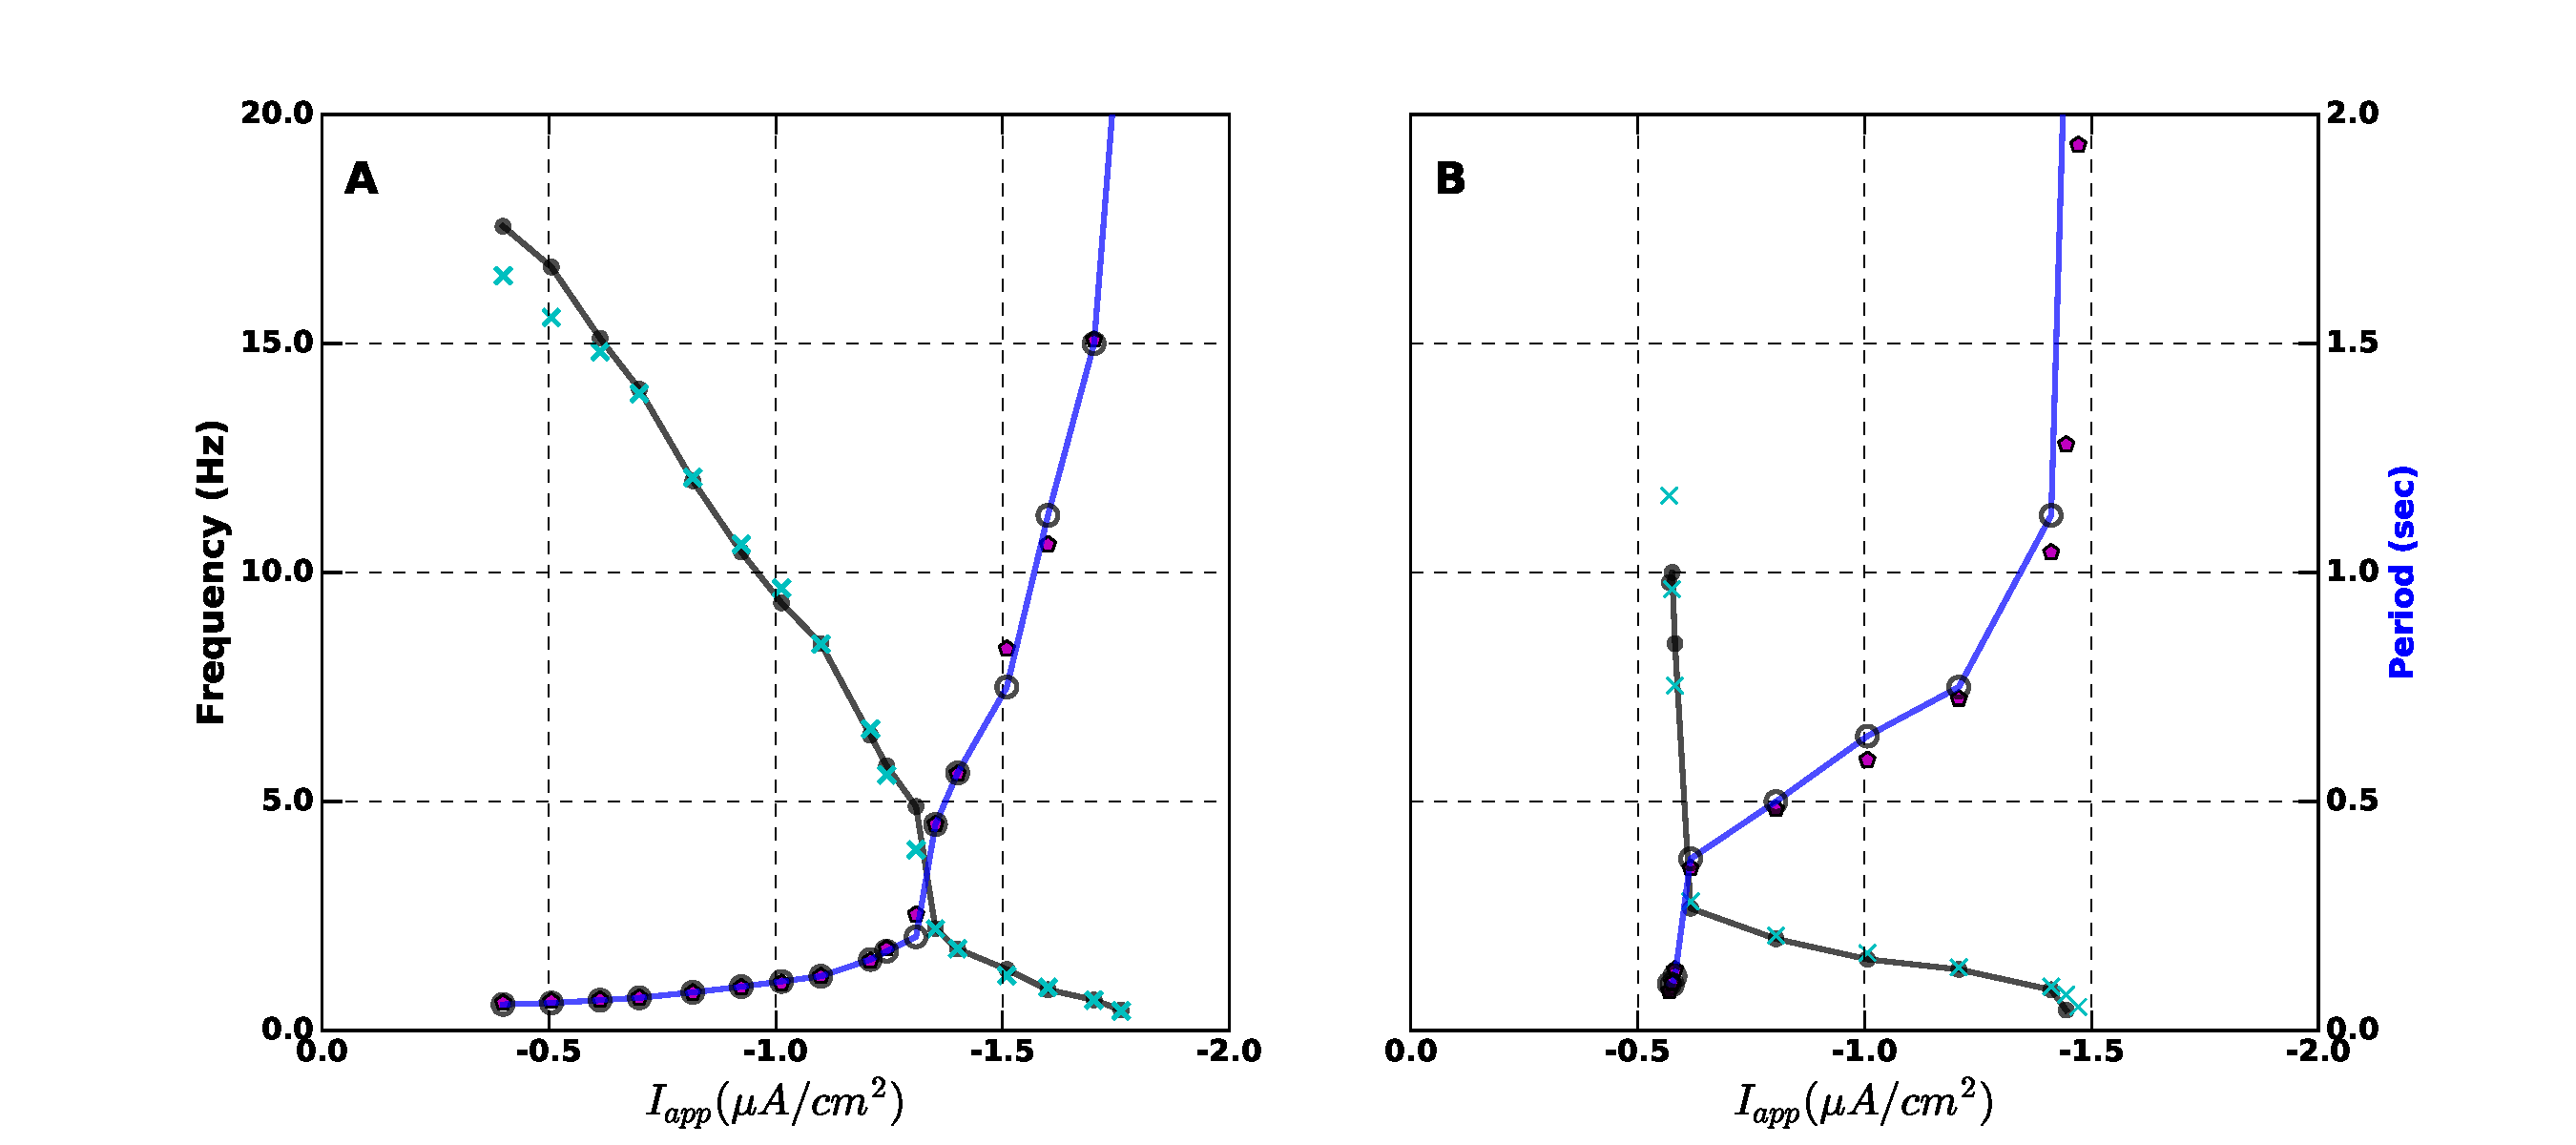
\includegraphics[width=1.0\textwidth, left]{figs/Figure6.pdf}
    \caption{{\bfseries \sffamily Frequency and period versus steady input 
    current.} This figure illustrates how an external current (ranging
    from $0$ to $-2\, \Rm{\mu A/cm^2}$ affects the bursts frequency (bursting
    mode) of the model. Black curve indicates frequency (black dots) in
    $\Rm{Hz}$ and blue curve period (white circle discs) in $\Rm{sec}$. 
    Cyan crosses (frequency) and magenta pentagons (period) indicate original
    data extracted from \cite{wang:1994}.}
    \label{Fig:6}
\end{figure}
%%

Fig~$2$ of \cite{wang:1994} illustrates an ``intermittent'' phase-locking
phenomenon, generated by integrating the model described in Table~\ref{Table:4}
and using a periodic pulse with frequency $10\,\Rm{Hz}$ and ratio 
$\frac{p}{P_0} = 0.8$ as external current. We applied the same protocol on 
the current implementation by using six different amplitude values and two 
different T-type calcium conductance values. 
$I_{app} = -1.4, -1.5, -1.6\, \Rm{\mu A /cm^2}$ and $g_T = 0.3\, \Rm{mS/cm^2}$
$I_{app} = -1.2, -1.5, -1.8\, \Rm{\mu A/cm^2}$ and  $g_T = 0.25\,
\Rm{mS/cm^2}$. After counting sub- and supra-threshold spikes, we computed the
symbolic patterns for every simulation. Figure~\ref{Fig:7} shows $2$ seconds
of membrane potential for every simulation along with symbolic patterns of $0$
(dark circles) and $1$ (green line segments). Results given in 
Figure~\ref{Fig:7} are similar to the ones of Fig~$2$A and Fig~$2$B.
%%
\begin{figure}[!htbp]
    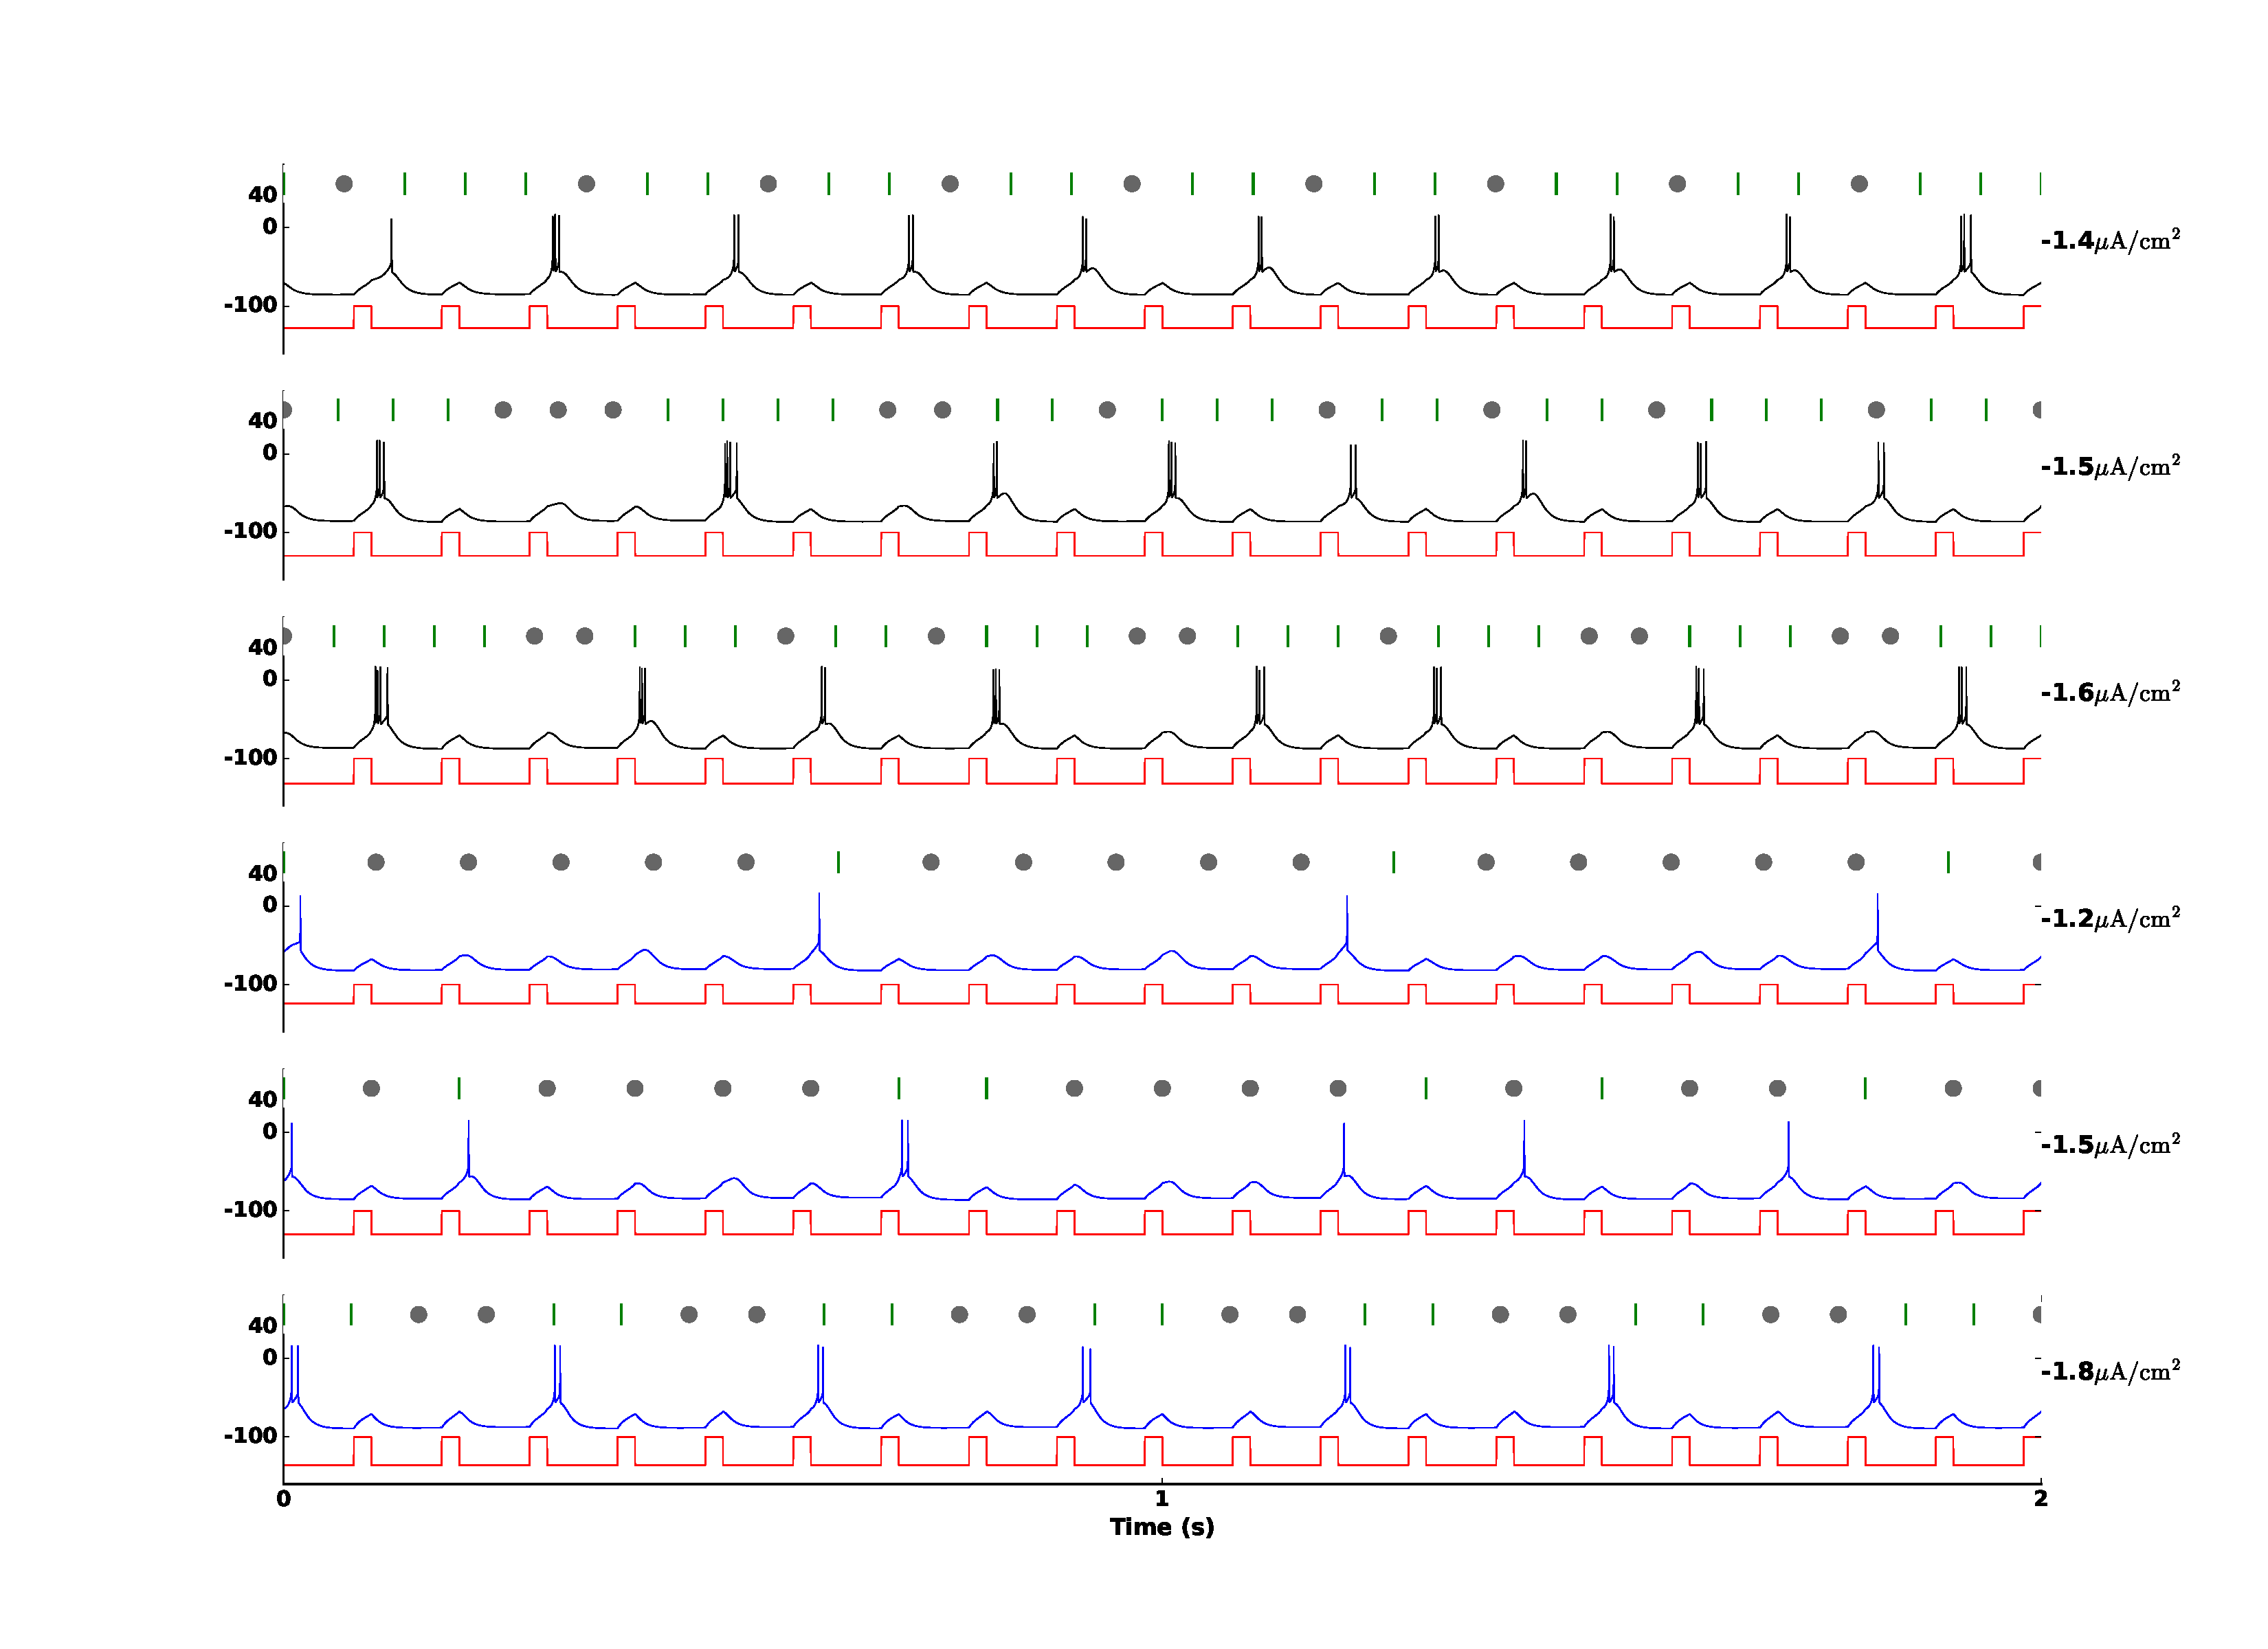
\includegraphics[width=1.1\textwidth]{figs/Figure7.pdf}
    \caption{{\bfseries \sffamily Symbolic patterns.} Six different simulations
    are illustrated here ($I_{app} = -1.4, -1.5 -1.6 \, \Rm{\mu A/cm^2}$
    with $g_T = 0.3\, \Rm{mS / cm^2}$) and ($I_{app} = -1.2, -1.5, -1.8\,
    \Rm{\mu A / cm^2}$ with $g_T = 0.25\, \Rm{mS / cm^2}$). Symbolic patterns
    are illustrated above membrane potential traces as green line segments -- 
    suprathreshold spikes and dark circles -- subthreshold spikes. Red curve 
    indicates the input periodic pulses.}
    \label{Fig:7}
\end{figure}
%%

\section{Conclusion}
\label{conclusion}

A conductance-based model for relay thalamocortical neurons proposed 
by \cite{wang:1994} was implemented in Python. The present model was tested 
thoroughly by using several examples from the original article. In general, 
the original model is easily implemented since all the equations and most
of the parameters (except the initial time step of the integration method) are
given. However, in some experimental protocols important information is
missing (e.g.\@ Wang's Fig~$1$ in \cite{wang:1994}, where our results do not
match exactly the original ones), leading to a less faithful reproduction of
those results. Furthermore, to the best of our knowledge, no any other
implementation of \cite{wang:1994} is available the thus we cannot compare
the current implementation to any other. 

{\sffamily \small
  \printbibliography[title=References]
}
\end{document}
